%
% fig/quadtree.tex -- Quadtree-Unterteilung (3 Stadien)
%
% Nachbau der SVG-Abbildung: Startquadrat -> Vierteln & Zaehlen -> Verfeinern
%
\begin{figure}
\centering
\def\weylquadtreezeros{%
  \node[root] at (0.45,3.10) {};
  \node[root] at (1.10,3.10) {};
  \node[root] at (1.45,2.95) {};
  \node[root] at (0.45,2.20) {};
  \node[root] at (3.05,3.10) {};
  \node[root] at (2.10,2.20) {};
  \node[root] at (2.45,2.35) {};
  \node[root] at (1.25,1.20) {};
}
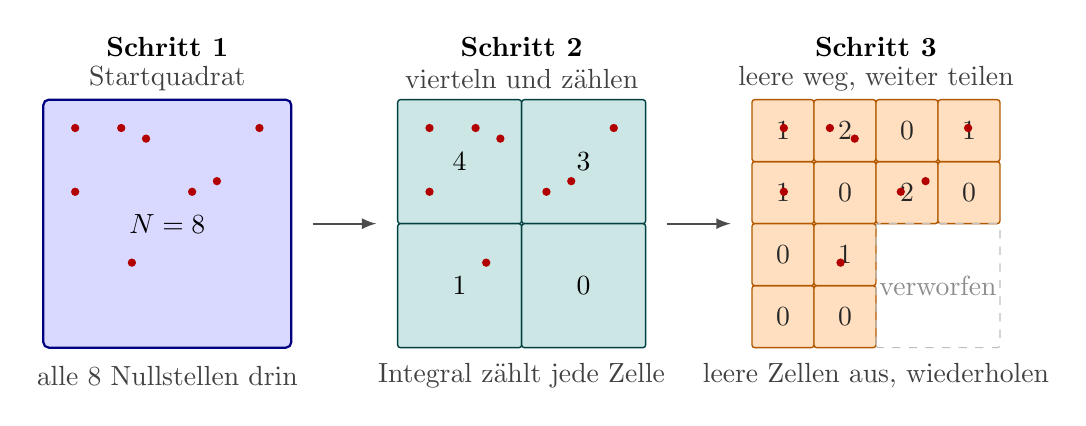
\begin{tikzpicture}[>=latex,thick,
    scale=0.9,
    stage1/.style={fill=blue!15,draw=blue!50!black,line width=0.8pt,rounded corners=2pt},
    stage2/.style={fill=teal!20,draw=teal!50!black,line width=0.5pt,rounded corners=1pt},
    stage3/.style={fill=orange!25,draw=orange!70!black,line width=0.5pt,rounded corners=1pt},
    discarded/.style={draw=gray!50,line width=0.4pt,dashed,rounded corners=1pt},
    root/.style={circle,fill=red!70!black,inner sep=0pt,minimum size=3pt},
    count/.style={font=\bfseries},
    cnt/.style={gray!30!black},
    stagelabel/.style={font=\bfseries},
    sublabel/.style={gray!50!black}]
%
% ============ STADIUM 1: Startquadrat ============
\begin{scope}[xshift=0cm]
  % Stadium-Labels
  \node[stagelabel] at (1.75,4.0) {Schritt 1};
  \node[sublabel] at (1.75,3.55) {Startquadrat};
  \begin{scope}[yshift=-0.25cm]
  % Grosses Quadrat
  \draw[stage1] (0,0) rectangle (3.5,3.5);
  % 8 Nullstellen, konsistent mit den Zählwerten der folgenden Stadien
  \weylquadtreezeros
  % Zentrale Zahl
  \node[count] at (1.75,1.75) {$N = 8$};
  \end{scope}
  % Unter-Beschriftung
  \node[sublabel] at (1.75,-0.65) {alle $8$ Nullstellen drin};
\end{scope}
%
% Pfeil 1
\draw[->,thick,gray!60!black] (3.8,1.5) -- (4.7,1.5);
%
% ============ STADIUM 2: Vierteln und Zählen ============
\begin{scope}[xshift=5cm]
  \node[stagelabel] at (1.75,4.0) {Schritt 2};
  \node[sublabel] at (1.75,3.55) {vierteln und zählen};
  \begin{scope}[yshift=-0.25cm]
  % 4 Quadrate (oben links: 4, oben rechts: 3, unten links: 1, unten rechts: 0)
  \draw[stage2] (0,1.75)    rectangle (1.75,3.5);   % oben links
  \draw[stage2] (1.75,1.75) rectangle (3.5,3.5);    % oben rechts
  \draw[stage2] (0,0)       rectangle (1.75,1.75);  % unten links
  \draw[stage2] (1.75,0)    rectangle (3.5,1.75);   % unten rechts
  % Nullstellen zum Nachzählen
  \weylquadtreezeros
  % Zahlen
  \node[count] at (0.875,2.625) {$4$};
  \node[count] at (2.625,2.625) {$3$};
  \node[count] at (0.875,0.875) {$1$};
  \node[count] at (2.625,0.875) {$0$};
  \end{scope}
  % Unter-Beschriftung
  \node[sublabel] at (1.75,-0.65) {Integral zählt jede Zelle};
\end{scope}
%
% Pfeil 2
\draw[->,thick,gray!60!black] (8.8,1.5) -- (9.7,1.5);
%
% ============ STADIUM 3: Verfeinern, leere weg ============
\begin{scope}[xshift=10cm]
  \node[stagelabel] at (1.75,4.0) {Schritt 3};
  \node[sublabel] at (1.75,3.55) {leere weg, weiter teilen};
  \begin{scope}[yshift=-0.25cm]
  % Oben links (war 4): 4 kleinere Quadrate mit 1 2 1 0
  \draw[stage3] (0,1.75)        rectangle (0.875,2.625);
  \draw[stage3] (0.875,1.75)    rectangle (1.75,2.625);
  \draw[stage3] (0,2.625)       rectangle (0.875,3.5);
  \draw[stage3] (0.875,2.625)   rectangle (1.75,3.5);
  \node[cnt] at (0.4375,3.0625) {$1$};
  \node[cnt] at (1.3125,3.0625) {$2$};
  \node[cnt] at (0.4375,2.1875) {$1$};
  \node[cnt] at (1.3125,2.1875) {$0$};
  % Oben rechts (war 3): 4 kleinere Quadrate mit 0 1 2 0
  \draw[stage3] (1.75,1.75)     rectangle (2.625,2.625);
  \draw[stage3] (2.625,1.75)    rectangle (3.5,2.625);
  \draw[stage3] (1.75,2.625)    rectangle (2.625,3.5);
  \draw[stage3] (2.625,2.625)   rectangle (3.5,3.5);
  \node[cnt] at (2.1875,3.0625) {$0$};
  \node[cnt] at (3.0625,3.0625) {$1$};
  \node[cnt] at (2.1875,2.1875) {$2$};
  \node[cnt] at (3.0625,2.1875) {$0$};
  % Unten links (war 1): 4 kleinere Quadrate mit 0 1 0 0
  \draw[stage3] (0,0)           rectangle (0.875,0.875);
  \draw[stage3] (0.875,0)       rectangle (1.75,0.875);
  \draw[stage3] (0,0.875)       rectangle (0.875,1.75);
  \draw[stage3] (0.875,0.875)   rectangle (1.75,1.75);
  \node[cnt] at (0.4375,1.3125) {$0$};
  \node[cnt] at (1.3125,1.3125) {$1$};
  \node[cnt] at (0.4375,0.4375) {$0$};
  \node[cnt] at (1.3125,0.4375) {$0$};
  % Unten rechts (war 0): verworfen, gestrichelt
  \draw[discarded] (1.75,0) rectangle (3.5,1.75);
  % Nullstellen zum Nachzählen
  \weylquadtreezeros
  \node[sublabel,opacity=0.6] at (2.625,0.875) {verworfen};
  \end{scope}
  % Unter-Beschriftung
  \node[sublabel] at (1.75,-0.65) {leere Zellen aus, wiederholen};
\end{scope}
%
\end{tikzpicture}
\caption{Drei Stadien von Weyls Algorithmus an einem Beispielpolynom mit $8$ Nullstellen.
Links das Startquadrat $D = [-r,r] \times [-r,r]$, das alle Nullstellen umschliesst.
Mitte: nach der ersten Iteration ist $D$ in vier Teilquadrate zerlegt, das
Wegintegral liefert die Nullstellenanzahl jedes Teilquadrats; in unserem Beispiel
$4$, $3$, $1$ und $0$ --- die Probe $4+3+1+0 = 8$ stimmt.
Rechts: das leere Quadrat (unten rechts) wird verworfen, die übrigen drei werden
ihrerseits geviertelt. Der Prozess wiederholt sich, bis jede Nullstelle in einem
eigenen kleinen Quadrat isoliert ist.
\label{weyl:fig:quadtree}}
\end{figure}
